\chapter{Proposed System}

\section{Introduction}
The proposed system is a web-based, multi-institution education management platform that brings the academic, administrative and communication work of colleges, universities and polytechnic institutes into one place and supports it with artificial intelligence. It responds to the problems identified in the previous chapters: scattered tools that keep the same records in several places, office staff who spend their time answering repeated questions, the need to protect sensitive student records, and the risk that an AI assistant may give answers that are not supported by any source.

The system lets many institutions register on one platform. Each institution works in its own isolated space, with its own users, roles, permissions, records and settings, and a platform-level Super Admin reviews registrations and manages subscriptions. Inside an institution, the system manages the academic structure, students, guardians and teachers, attendance, examinations and results, finance, hostel, library, human resources, inventory and notices. Students and guardians use a portal to see their own records, and every user can ask questions to a message and voice assistant in Bangla or English. A separate prediction service estimates academic risk and forecasts GPA.

The system is built from four applications: a Next.js frontend, a Core API that holds all business rules and is the only entry point for the frontend, an AI service for predictions, and a Voice service for language and speech processing. The expected benefits are that information is entered once and reused everywhere, each user sees only what their role allows, families can find answers without visiting the office, and the assistant never answers from guesswork.

\section{Proposed System}
The central idea of the proposed system is a single platform that holds all of an institution's records and uses them both for daily management and for answering people's questions. In place of separate registers and spreadsheets, each module of the system reads and writes the same student, teacher, guardian and staff records in one PostgreSQL database, so a student created in the academic module is the same student who is billed in finance, allocated a seat in the hostel, issued books in the library and answers questions through the assistant.

The overall structure of the system is shown in Figure~\ref{fig:architecture}. Users work through a web browser with the Next.js frontend. The frontend sends every request, with a signed JSON Web Token, to the Core API. The Core API, written in Node.js, Express and TypeScript, checks who the user is and what they may do, applies the business rules of each module, and reads and writes the database. Every record carries the identifier of its institution, and every query is limited to the signed-in user's institution. When a request needs prediction, the Core API calls the AI service; when it needs document reading, text embeddings, answer drafting or speech processing, it calls the Voice service. Both calls carry a shared service token. The Voice service uses a language model and an embedding model that run on the institution's own server through Ollama, and it writes call transcripts to the same database through its own restricted database login protected by row security policies. The Core API also sends email through an SMTP server for credentials, notices, receipts, reminders and forwarded questions.

\begin{figure}[htbp]
  \centering
  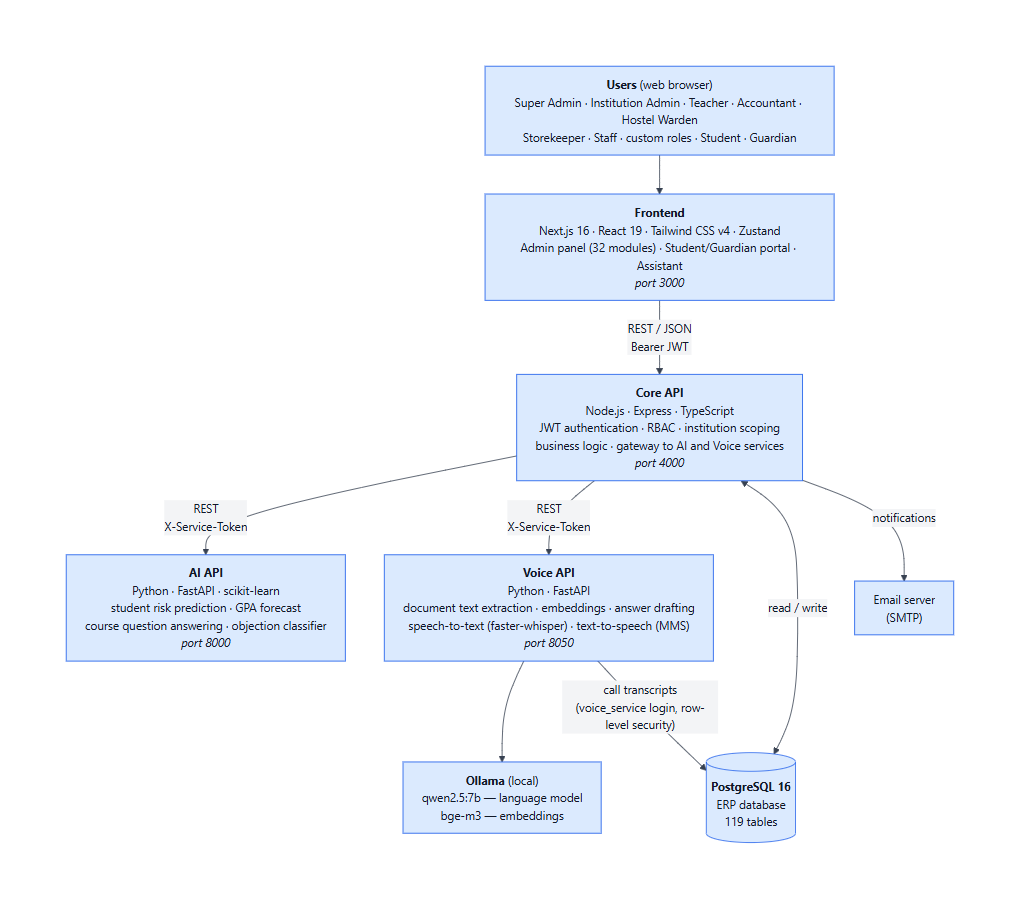
\includegraphics[width=\textwidth,height=0.85\textheight,keepaspectratio]{book_figures/fig01_system_architecture.png}
  \caption{Overall system architecture of the platform}
  \label{fig:architecture}
\end{figure}

People use the system through roles. The built-in roles are Super Admin, Institution Admin, Hostel Warden, Accountant, Storekeeper, Staff, Teacher, Student, Guardian and Not System User; institutions can also create their own roles with chosen permission keys. As shown in Figure~\ref{fig:roles}, administrators use the full administration panel, staff roles use the same panel but see only the modules their permissions allow, and students and guardians use the portal. A Not System User is a person kept on record, such as a contact, who cannot sign in.

\begin{figure}[htbp]
  \centering
  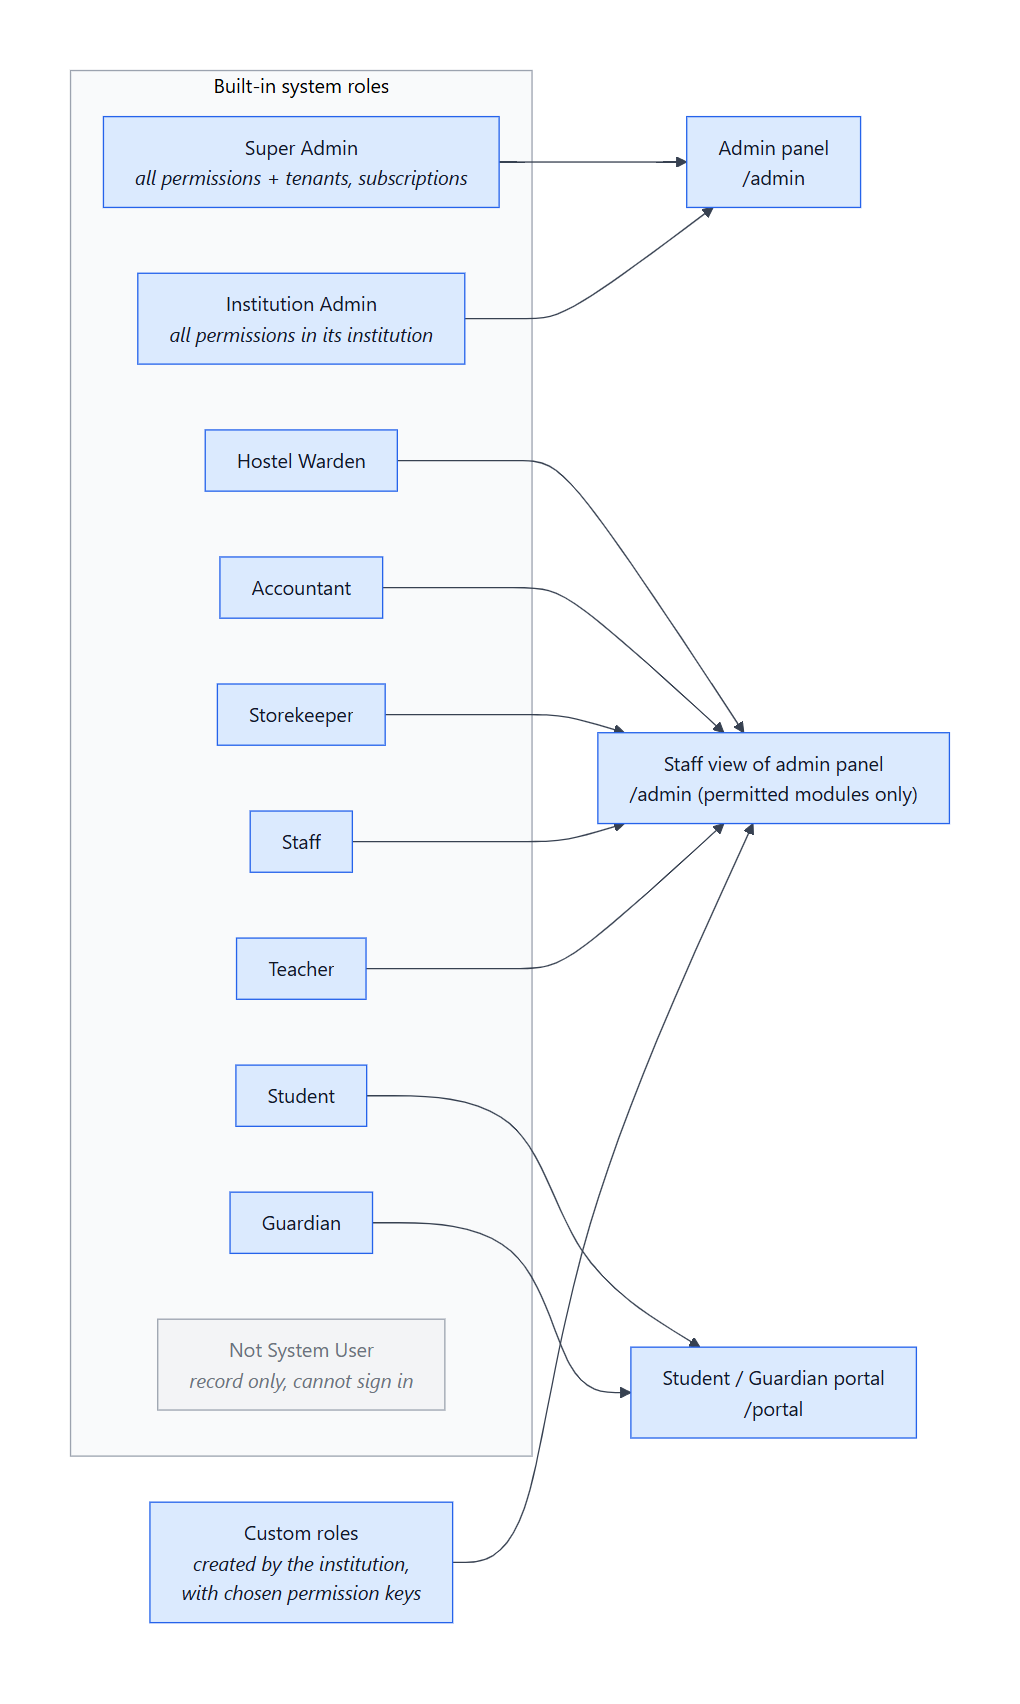
\includegraphics[width=0.75\textwidth,height=0.85\textheight,keepaspectratio]{book_figures/fig04_roles_portals.png}
  \caption{Built-in user roles and the portals they use}
  \label{fig:roles}
\end{figure}

The administration panel is organised into numbered modules, shown in Figure~\ref{fig:modules}. The modules for platform management, system and institution configuration, students, guardians, teachers, attendance, examinations, library, finance, human resources, hostel, inventory, notices, settings, payment integration and the AI message and voice assistant are connected to the Core API and work with live data. The remaining modules, such as learning management, classroom, scholarship, application, voting, research, certificate, transport, document, reports, notification centre, security centre, monitoring, workflow and data import and export, currently provide interface screens with built-in sample data and are planned to be connected in future work. The objection module has a working backend interface that the Voice service uses to file tickets, while its screens are not yet connected.

\begin{figure}[htbp]
  \centering
  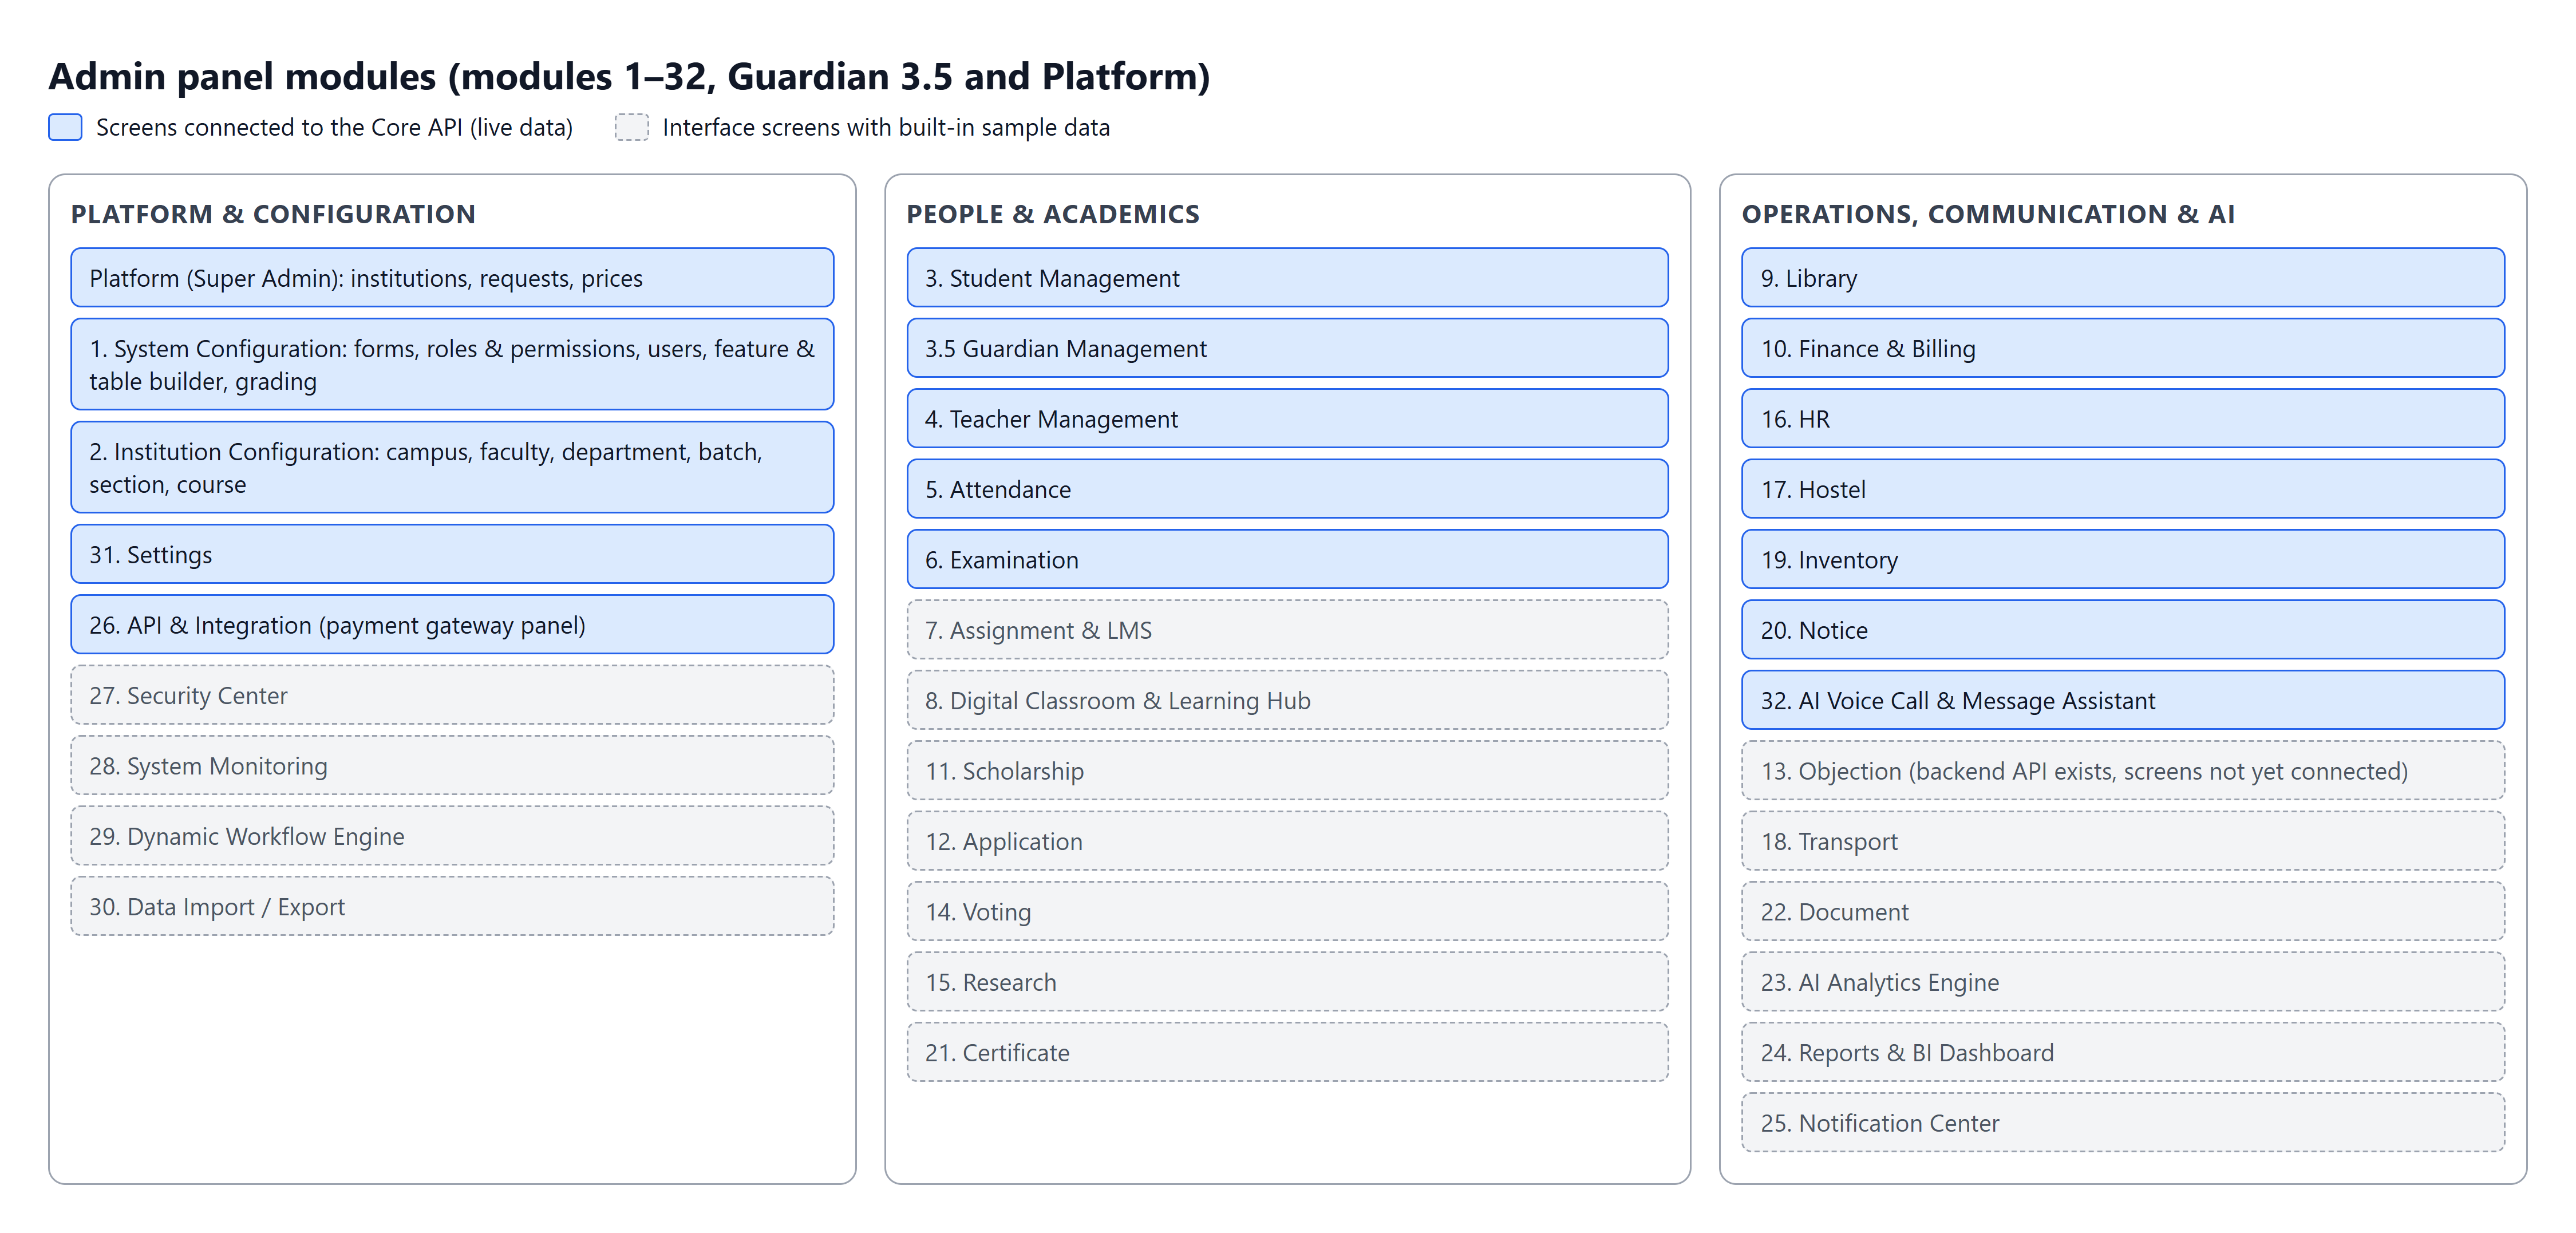
\includegraphics[width=\textwidth,height=0.85\textheight,keepaspectratio]{book_figures/fig03_module_map.png}
  \caption{Admin panel module map and integration status}
  \label{fig:modules}
\end{figure}

Some work in the system runs automatically in the background. A hostel scheduler generates rent invoices, sends upcoming and overdue rent reminders, generates subscription invoices, reconciles online payments and delivers queued notifications; each job can be repeated safely and catches up after downtime, and a database advisory lock prevents two servers from running the same job at once. An inventory scheduler sends one daily alert digest per institution. An assistant scheduler processes uploaded documents and retries forwarded questions that could not be delivered.

Compared with keeping separate tools, the proposed system removes repeated data entry, applies the same security checks to every module, and turns the institution's own records and documents into answers that students, guardians and staff can get at any time.

\section{Features of the Proposed System}
The proposed system consists of several features that work together to cover the daily work of an institution while keeping its data secure and separate from other institutions. Each feature reads and writes the same central records, is protected by the same authentication and permission checks, and is limited to the signed-in user's institution. The features are described below.

\subsection{Multi-Institution Registration and Subscription}
An institution joins the platform through a public registration page. It can view the available plans, choose the modules it needs and a monthly or yearly billing cycle, and receive a price quote before submitting its registration. A new registration remains pending until the Super Admin reviews it; until then, its users cannot sign in. The Super Admin can approve or reject registrations and subscription change requests, view each institution's overview and activity, suspend or reactivate an institution, change the modules it can use, set module prices and resend the institution administrator's credentials.

The platform also manages subscription billing. Invoices are generated for each institution's billing period, with a due date ten days after issue, and yearly subscriptions are charged for ten months. Payments can be recorded by bank transfer, bKash, Nagad, cash, cheque or card, and an invoice shows as unpaid, partially paid, paid, overdue or void. An institution administrator can see the institution's own subscription and request changes. This feature makes it possible to offer the same system to many institutions while keeping each one's data and modules separate.

\subsection{User, Role and Permission Management}
This feature controls who can use the system and what each person can do. Administrators create user accounts and link them to student, teacher, guardian or staff records. When an account that can sign in is created, the system generates a temporary password and sends it only to the person's own email; it is never shown or logged. The person must choose a new password on first sign-in, and until they do, the system allows only the password change.

Passwords are stored as bcrypt hashes. After five wrong passwords an account is locked for fifteen minutes, and each failed or successful sign-in is recorded in the account's activity. Sessions use signed JSON Web Tokens that last eight hours, or fifteen minutes for a temporary password, and on every request the Core API reloads the user, role and institution status from the database, so a disabled account, a changed role, a suspended institution or maintenance mode takes effect immediately.

Permissions are organised as a tree of features and actions, for example reading, creating, updating, approving or exporting records in each module. Built-in roles have fixed permissions and cannot be edited or deleted, while institutions can create, clone and edit their own roles, attach a registration form to a role, and give individual users permission overrides. Administrators can reset passwords, assign wards to guardians, review each user's activity and read the institution's audit log.

\subsection{Dynamic Form, Feature and Table Builders}
Institutions often need to collect information that a fixed system did not plan for. The form builder lets an administrator design forms with text, long text, email, phone, number, date, select, radio, checkbox and multi-select fields, and fields can be shown only when an earlier answer meets a condition. A form is published as a version; editing a published form starts a new draft version, and earlier answers keep the version they were given in. Submitted answers are checked against that version, and answers to hidden fields are discarded.

The feature builder uses these forms to add new record types inside any module. Each feature has its own form and its own read, create and update permissions, and once published it appears in the navigation of the users allowed to open it, who can then add, edit and delete its records. The table builder lets administrators define table layouts with their own columns and choose whether they can be exported. The same configuration area holds the academic grading configuration, with the grade ranges, letter grades, grade points, pass marks and GPA scale used when results are calculated, and the institution's settings sections.

\subsection{Academic Structure and People Management}
This feature models the academic organisation of an institution. Administrators manage departments, programs, academic sessions, sections, courses and classes, where a class links a course and a section to a teacher. Campus information and institution metadata are also kept.

Student records include the student number, personal and contact details, program and section, admission date, status and guardian details. Students can be moved between sections and programs together, their status can be changed with a reason, and a portal account can be created for a student and for the student's guardian in one step. Teacher records include the employee number, department, designation and qualification, and a teacher can also be given an account. Guardian accounts are linked to one or more students, which controls whose records a guardian can see in the portal.

\subsection{Attendance, Examination and Results}
Teachers see the classes they teach and take attendance for each class meeting on an attendance sheet, marking each student's status with an optional note. An attendance report shows each student's record for the class.

Examinations are created for each academic session with a name, weight and default maximum marks. For each class, an exam has an assessment in which marks are entered, with absent students marked separately. An assessment can be locked to stop further changes and unlocked when a correction is needed. Class results combine the weighted assessments into a percentage for each student, and the grading configuration converts it into a letter grade and grade point and decides whether the student passed. Results are published to students and guardians by a user with approval rights, and only when the weights of the session's exams add up to 100\% and the marks of every exam are locked; a published result can be withdrawn. In the portal, results are shown term by term with a GPA for each term weighted by course credits.

\subsection{Finance and Billing}
The finance feature manages student fees. Administrators define fee heads and a fee structure that sets the amount of each fee for programs. Invoices can be created one by one or generated for many students at once; each invoice records its items, due date and total, and can be adjusted or cancelled with a reason. Payments are recorded against invoices with a method, reference and receipt number, protected against being recorded twice, and can be reversed with a reason. A statement shows every invoice and payment of a student, and a summary shows collection figures and targets for the institution. Students and guardians see their fees and invoices in the portal.

\subsection{Hostel Management}
The hostel feature covers the full life of a hostel resident. Wardens manage buildings, rooms and seats, including bulk room creation and room status. Wardens create an allocation for a student, which starts as pending and is then assigned to a seat, rejected or later vacated, with documents attached to it. Rent settings define rent and due days per building or seat, and every change is recorded. Rent invoices are generated automatically each period, can be adjusted, and are paid at the desk or online. For online payment, an invoice can produce a payment link that a student or guardian opens without signing in and pays through a configured bKash gateway; the result is reconciled automatically, and gateway transactions can be verified by staff. Receipts are available on screen, as PDF documents and by email, and payments can be reversed.

Beyond rent, the feature tracks due rent with export, sends reminders and notifications by email or SMS through configurable templates with retry, manages additional hostel fees and fee groups assigned to students, and handles refunds. Meals are published with a menu and image, students book or cancel meals from the portal, staff mark meals as collected, and meal dues can be reminded. Visitors are registered with documents and a ticket and are checked in and out. Maintenance tickets record room problems and their progress, and a ledger and audit log show every financial change for an allocation.

\subsection{Library Management}
The library feature keeps the book catalogue with the number of copies of each book and the library's lending settings. Library staff issue books to borrowers, renew loans and record returns. Fines for late return are recorded on the loan; taking fine money is desk work, while waiving a fine needs approval permission. Borrowers see their own loans, and students and guardians see library loans in the portal.

\subsection{Human Resources}
The human resources feature keeps staff records and salary details for teachers and other staff. Administrators define leave types, and leave requests are created, approved or rejected, and cancelled, with leave balances for each person. Payroll runs are created for a period, approved and then marked as paid, producing payslips. Teachers and staff have self-service access to their own leave balances, can request or cancel leave, and can see their own payslips.

\subsection{Inventory and Asset Management}
The inventory feature manages stores and the items they hold, including item categories, bulk import of items, archiving and restoring. Every stock change is recorded as a movement: receiving, issuing, returning, counting, writing off, consumption and wastage, and a movement can be reversed. Stock can be transferred between stores through a request that is approved or rejected and then received. Items can be tracked in batches.

Purchasing is supported with suppliers and purchase orders that are approved, received, closed or cancelled. Staff in other departments request items through requisitions, which are approved, issued and received. Assets are registered or created from stock and move through clear states: they can be assigned and returned, sent for repair and marked repaired, reported lost and found, moved, or disposed of, where disposal needs approval permission. Every action is kept in the asset's history. For the hostel kitchen, daily meal counts and kitchen use are recorded per day and month. Reports show expenses and items that need to be reordered, a movement analysis shows how stock is used, and low-stock alerts are shown in the panel and sent as a daily email digest.

\subsection{Notice Management}
Administrators write notices and target them to everyone, students, guardians, teachers or staff. A notice is kept as a draft until it is published, can be archived later, and can also be sent by email to its recipients. Before sending, the list of recipients for the chosen audience can be reviewed. Each signed-in user sees a notice feed containing only the notices meant for their audience, and students and guardians see notices in the portal.

\subsection{Student and Guardian Portal}
The portal gives students and guardians a single page for their own information. It shows the student's profile, academic results and attendance, fees and invoices, notices and library loans. Hostel residents can pay rent invoices online, see the meal menu, and book or cancel meals. A guardian sees the records of the students linked to their account. Every portal request returns only the records that belong to the signed-in student or to the guardian's linked students.

\subsection{AI Message and Voice Assistant}
The assistant answers questions from students, guardians and staff in Bangla or English, typed or spoken. It first decides what kind of question it is. A request to change data is politely refused and recorded in the audit log. A question about the asker's own records, such as meal count, meal menu or time, attendance, result, fees due or application status, is answered directly from the database for that person only. Any other question is answered from the institution's knowledge: documents uploaded by administrators and answers previously approved by an administrator. These are searched by shared words and by meaning using bge-m3 embeddings, and the locally hosted qwen2.5:7b language model writes an answer using only the passages found and cites them. If the language model is not available, the assistant returns an approved answer or document text only when the match is strong enough.

When no trusted answer is found, the assistant does not guess. It forwards the question to the responsible person whose topics best match the question, or to the default person, by SMS, email, call or the person's own panel, with a private reply link that is valid for fourteen days. Failed deliveries are retried up to five times. The reply goes to an administrator for review together with an AI-drafted version; only after approval does it become part of the knowledge base and answer future questions. Users can rate answers, and administrators see analytics of how questions were answered.

The voice channel lets a user hold a spoken conversation in the browser. Each spoken turn is converted to text with faster-whisper, answered through the same process as a typed question, and read aloud with MMS Bangla or English voices. Every call and turn is stored, and administrators can review call transcripts.

\subsection{AI Prediction Service}
The prediction service provides two models through the Core API. The first is a Random Forest classifier that takes a student's attendance rate, midterm average, assignment submission rate, previous CGPA and days of overdue fees, and returns a risk probability with a level of low, medium, high or critical, the factors that raised the risk and recommended actions for staff. The second is a ridge regression model that takes the current CGPA, term credits, quiz average and midterm marks, predicts the term GPA and returns the projected CGPA with a range and a trend. The service also offers course question answering and a classifier for objections written in Bangla or English. In the current version, both prediction models are trained on synthetic data generated when the service starts, so their output demonstrates the integration of prediction into the platform rather than validated accuracy.

\section{Summary}
This chapter described the proposed system: a multi-institution education management platform built from a Next.js frontend, a Core API, an AI service and a Voice service that share one secure entry point and one central database. It explained how users reach the system through roles and portals, how modules share the same records, and which modules work with live data. It then described the main features: multi-institution registration and subscription, user and permission management, dynamic form, feature and table builders, academic structure and people management, attendance, examinations and results, finance, hostel, library, human resources, inventory, notices, the student and guardian portal, the AI message and voice assistant, and the prediction service. Together these features meet the objectives set in Chapter~I, and the following chapters present the requirements, methodology, design and implementation of the system.
